\documentclass[conference]{IEEEtran}
\IEEEoverridecommandlockouts
% The preceding line is only needed to identify funding in the first footnote. If that is unneeded, please comment it out.
\usepackage{cite}
\usepackage{amsmath,amssymb,amsfonts}

\usepackage{graphicx}
\usepackage{textcomp}
\usepackage{xcolor}
\usepackage{amsmath, amssymb, amsthm}
\usepackage{algorithm}
\usepackage{algpseudocode}
\usepackage{booktabs}
\usepackage{hyperref}
\newtheorem{lemma}{Lemma}
\newtheorem{proposition}{Proposition}
\newtheorem{corollary}{Corollary}
\newtheorem{theorem}{Theorem}
\newtheorem{example}{example}
\newtheorem{remark}{Remark}
\newtheorem{assumption}{Assumption}
\newtheorem{definition}{Definition}
%\def\BibTeX{{\rm B\kern-.05em{\sc i\kern-.025em b}\kern-.08em
%    T\kern-.1667em\lower.7ex\hbox{E}\kern-.125emX}}
\begin{document}

% For draft editing
\newcommand{\Red}[1]{\textcolor{red}{[{#1}]}}

\title{\LARGE \bf
Evolutionary Algorithms for Actuator-Sensor-Communication Co-Design in Distributed Control
}
\author{Pengyang Wu and Jing Shuang (Lisa) Li% <-this % stops a space
\thanks{At the time this manuscript was written, P.W. and J.S.L. were both with the Department of Electrical Engineering and Computer Science, University of Michigan, Ann Arbor, MI, 48109, USA.
        {\tt\small \{pengyanw, jslisali\}@umich.edu}.    }%
}

\maketitle

\begin{abstract}
This paper studies the co-design of actuators, sensors, and communication in the distributed setting, where a networked plant is partitioned into subsystems each equipped with a sub-controller interacting with other sub-controllers. The objective is to jointly minimize control cost (measured by LQ cost) and material cost (measured by the number of actuators, sensors, and communication links used). We approach this using an evolutionary algorithm to selectively prune a baseline dense LQR controller. We provide convergence bounds, performance bounds, and probabilistic stability guarantees for this algorithm. For unstable plants, controller pruning is more likely to induce instability; we provide an algorithm modification to address this. The proposed methods is validated in simulations. One key result is that co-design of a 98-state swing equation model can be done on a standard laptop in seconds; the co-design outperforms naive controller pruning by over 50\%.
\end{abstract}

\section{Introduction}
Large-scale networked dynamical systems arise in a wide range of modern engineering applications, including power grids, traffic networks, multi-agent robotic systems, and cyber-physical infrastructures. In such systems, centralized control architectures are often impractical due to scalability limitations and communication constraints. These challenges have motivated extensive research on \emph{distributed control}, where control actions are computed using only local information and limited inter-agent communication \cite{9535262, anderson2019system, shin}. In parallel, practical deployments increasingly demand \emph{co-design} methodologies that jointly consider control performance, sensor and actuator placement, and communication structure. Despite significant progress, \emph{distributed controller co-design} remains a fundamental but underexplored problem due to its nonconvex combinatorial nature. Existing work have attempted to address part of the codesign problem\cite{pequito2015minimum}. Sparsity-promoting optimal control \cite{9535262} introduce convex relaxations to encourage sparse feedback gains optimization. However, it relies on the Quadratic Invariance(QI) property of the problem\cite{9535262}. The LQRSP \cite{lqrsp} method simultaneously identifies sparse communication topologies and optimizes $H_2$ performance, yet lacks convergence and stability guarantees for the nonconvex LQR cost. 

 Another representative line of work in \emph{distributed controller co-design} studies the simultaneous sensor and actuator selection problem (SSASP)\cite{Nugroho2019Automatica}, where the objective is to identify a minimal set of sensing and actuation nodes that render a large-scale dynamical network stabilizable. While these methods provide valuable insights into joint actuator-sensor design, they primarily focus on stabilization feasibility, which doesn't take into account the controller performance optimization and can limit scalability in high-dimensional systems. Complementary to this algorithmic perspective, structural and graph-theoretic approaches have been proposed to study control and communication co-design at an abstract level. For instance, \cite{Nugroho2019Automatica} investigates the joint selection of actuators, sensors, and control configurations using structural system theory, and establishes fundamental complexity limits for such co-design problems. 
 
 While these methods have yielded valuable insights, they typically decouple structure selection from controller synthesis, rely on convex surrogates that may be conservative for real systems\cite{Regularization}, or face scalability limitations in large-scale networks. As a result, a general and flexible framework for distributed control co-design that simultaneously explores structural and control dimensions remains elusive. In this letter, we introduce the Evolutionary Algorithm(EA) based algorithm to co-design the controller of a discrete linear system and optimize on both the sparsity and control performance. EA has been widely applied to complex search problems, with their search effectiveness demonstrated in neural architecture search~\cite{EA-survey} and their computational complexity characterized through rigorous runtime analysis via fitness-level lower bound methods~\cite{EAtime}.


\section{Problem Setup: sparse LQR Co-Design via Evolutionary Algorithm}

Consider a discrete-time linear time-invariant system:
\begin{equation} \label{eq:plant}
x_{k+1} = A x_k + B u_k
\end{equation}
where $x_k \in \mathbb{R}^{N_x}$ is the state vector, $u_k \in \mathbb{R}^{N_u}$ is the control input, $A \in \mathbb{R}^{N_x \times N_x}$ is the state matrix, and $B \in \mathbb{R}^{N_x \times N_u}$ is the input matrix.
We seek a sparse state-feedback controller $K_{\text{s}} \in \mathbb{R}^{N_u \times N_x}$ such that plant \eqref{eq:plant} evolving under controller $u_k = K_{\text{s}} x_k$ satisfies some control objective.

We consider designing $K_{\text{s}}$ to jointly minimize the number of actuators, sensors, and communication links, as well as the LQ control cost. 
The optimization vector $\theta$ is defined to represent the controller's sparsity structure. Since $Q$ and $R$ are fixed, we define:
\begin{equation}
\theta = [\,\ell, \;\mathbf{a}, \;\mathbf{s}\,]
\end{equation}
where:
\begin{enumerate}
    \item[(a)] $1 \leq \ell \leq N_u N_x$ is an integer gene determining the number of nonzero elements in $K_\mathrm{s}$;
    \item[(b)] $\mathbf{a} \in \{0, 1\}^{N_u}$ is a binary mask vector representing the selection of active actuators;
    \item[(c)] $\mathbf{s} \in \{0, 1\}^{N_x}$ is a binary mask vector representing the selection of active sensors.
\end{enumerate}

We formulate the sparse controller co-design problem as a mixed-integer combinatorial optimization problem. The objective is to find the optimal sparsity configuration variables (e.g., actuator/sensor selections $\mathbf{a}$ and $\mathbf{s}$) and the controller $K_\mathrm{s}$ that minimize a weighted combination of control performance and sparsity cost:
$$\begin{aligned}
\min_{K, \theta} \quad & F(K_{\text{s}}, \theta) = \frac{J_{\text{perf}}(K_{\text{s}})}{J_{\text{BM}}} +  \phi(K_{\text{s}}) \\
\text{s.t.} \quad & \rho(A + B K_{\text{s}}) < 1 
\end{aligned}$$
where: (a) $J_{\text{perf}}(K)$ is the generalized $\mathcal{H}_2 / \mathcal{H}_\infty$ performance. (b) $J_{\text{BM}}$ is the benchmark(optimal) cost of the initial controller. (c) $\phi(K)$ represents the sparsity penalty, such as the $\ell_0$-norm (the number of non-zero elements, $\|K\|_0$) or the total number of active actuators and sensors ($\|\mathbf{a}\|_0 + \|\mathbf{s}\|_0$). (d) $\alpha \ge 0$ is the trade-off coefficient that dictates the relative importance of sparsity versus control performance.

A common measure for controller performance loss is the Linear Quadratic Regulator (LQR) cost: Assuming the initial state $x_0$ is a random variable drawn from a Gaussian distribution $x_0 \sim \mathcal{N}(0, X_0)$. Under this assumption, the expectation expression for $J_{\text{LQR}}(K)$ is defined as the expected value of the infinite-horizon quadratic cost:$$J_{\text{LQR}}(K) = \mathbb{E}_{x_0} \left[ \sum_{t=0}^{\infty} \left( x_t^\top Q x_t + u_t^\top R u_t \right) \right]$$
where $Q \succeq 0$ and $R \succ 0$.
\subsection{Co-design via LQR pruning}

In this paper, we perform co-design by pruning the optimal (but dense) LQR controller (i.e., replacing terms with zeros). This approach is motivated by the methodology in \cite{shin}.

First, we compute the baseline controller $K_{\mathrm{d}}$, which represents the optimal dense LQR solution for the unconstrained centralized system. The sparse controller is then derived by pruning $K_{\mathrm{d}}$ according to the parameter $\theta$. Specifically, the sparse gain matrix is obtained as:
\begin{equation} \label{eq:ks}
K_\mathrm{s}(\theta) = \Pi_{a,s} \left( \text{trunc}(K_{\mathrm{d}}, \ell) \right)
\end{equation}
where $\text{trunc}(K_{\mathrm{d}}, \ell)$ denotes the operator that keeps the $\ell$ largest-magnitude entries of $K_{\mathrm{d}}$ and sets the remaining entries to zero. Here, the integer $1 \leq \ell \leq N_u N_x$ represents the desired number of active control links to be retained from the dense benchmark. The projection operator $\Pi_{\mathbf{a},\mathbf{s}}(\cdot)$ enforces hardware constraints by nullifying all feedback links associated with inactive actuators and sensors, as indicated by the zero entries in the binary masks $\mathbf{a}$ and $\mathbf{s}$.

\begin{equation}
\label{cost_ea}
\begin{aligned}
J_{\text{EA}}(\theta) 
&= \frac{J_{\text{LQR}}(K_{\text{s}}(\theta))}{J_{\text{BM}}} \\
&\quad + \left(
w_c \|K_{\text{s}}\|_0
+ w_a \|a\|_1
+ w_s \|s\|_1
\right).
\end{aligned}
\end{equation}
where $w_c, w_s, w_a$ are positive constants representative of co-design penalty. The optimization objective is:
\begin{equation}
\begin{aligned}
\min_{\theta} \quad & J_{\text{EA}}(\theta) \\
\text{s.t.} \quad &  1 \leq \ell \leq N_u N_x, \\
&\theta = [\,\ell, \;\mathbf{a}, \;\mathbf{s}\,], \\
& a_j \in \{0, 1\}, \quad j = 1, \dots, N_u, \\
& s_i \in \{0, 1\}, \quad i = 1, \dots, N_x, \\
\text{where} \quad & K_\mathrm{s}(\theta) = \Pi_{\mathbf{a},\mathbf{s}} \left( \text{trunc}(K_{\mathrm{d}}, \ell) \right).
\end{aligned}
\label{eq:optimization_problem}
\end{equation}

\section{Evolutionary Algorithm for sparse LQR Co-Design}
The optimization problem \eqref{eq:optimization_problem} is nonconvex and combinatorially difficult. To solve this, we will use an evolutionary algorithm (EA) based method. Rather than enforcing a fixed sparsity pattern or relying on convex relaxations, EA treats the co-design problem as a population-based dynamic search over both controller parameters and sparsity parameter $\theta$. EA is particularly advantageous as it avoids the need for differentiable and continuous functions, thus naturally handling mixed discrete–continuous combinatorial search and admitting flexible objective formulations. 

The process is shown in Algorithm \ref{alg:ea}. Here, the EA is governed by five key parameters: population size $N_p$, maximum generations $G_{\max}$, elite count $n_e$, crossover probability $p_c$, and mutation probability $p_m$. The population is initialized by drawing the hardware masks $\mathbf{a}$ and $\mathbf{s}$ from a  Bernoulli distribution, while $\ell$ is set to match the number of non-zero elements in the baseline $K_{\mathrm{d}}$. In each generation, the individuals $\theta = [\,\ell, \;\mathbf{a}, \;\mathbf{s}\,]$ are ranked by ascending fitness. The top $n_e$ elite individuals—those achieving the lowest cost $J_{EA}$—are carried over unchanged. Then, we apply the update steps for $\theta$:

The EA is driven by the following three functional operators:\begin{enumerate}\item \textbf{Selection:} The operator $\text{Selection}(\mathcal{P}_t, \tau)$ returns a parent ${\theta_{p1}, \theta_{p2}}$ sampled from population $\mathcal{P}_t$ according to the probability:\begin{equation}P(\theta_i) = \frac{\exp(-F(\theta_i)/\tau)}{\sum_{\theta_j \in \mathcal{P}_t} \exp(-F(\theta_j)/\tau)}\end{equation}where $F(\theta_i)$ represents the fitness cost and $\tau$ is the temperature parameter.
\item \textbf{Crossover:} The operator $\text{Crossover}(\theta_{p1}, \theta_{p2}, p_c)$ generates a child $\theta_{c}$ via a single-point split at $k \sim \mathcal{U}(1, |\theta|-1)$:
\begin{equation}
    \text{Crossover}(\theta_{p1}, \theta_{p2}, p_c)_i = 
    \begin{cases} 
    \theta_{p1, i}, & i \le k \\ 
    \theta_{p2, i}, & i > k 
    \end{cases}
\end{equation}

\item \textbf{Mutation:} The operator $\text{Mutation}(\theta_{c}, p_m)$ produces a mutated individual $\theta_{\text{new}}$ through stochastic perturbations:
\begin{equation}
    \text{Mutation}(\theta_{c}, p_m, d) = 
    \begin{cases}
    \mathbf{v}_{c} \oplus \mathbf{m}, \mathbf{v} \in \{\mathbf{a}, \mathbf{s}\} \\
    \text{proj}(\ell_c + \delta), \delta \sim \text{Unif}\{-d, d\}\\
    m_j \sim \text{Ber}(p_m)
    \end{cases} 
\end{equation}
where $\text{proj}(\cdot)$ denotes the saturation function that clips the value of $\ell$ within its permissible bounds $[1, N_u N_x]$, and
$\oplus$ denotes the element-wise XOR operation.

\end{enumerate}

As shown in Algorithm~\ref{alg:ea}, throughout evolution, the minimum cost, average cost, and ratio of unstable to stable
individuals are recorded. After $G_{\max}$ generations, the best-performing individual is returned. Simulations showing Algorithm~\ref{alg:ea}'s effectiveness are shown in
Section~\ref{simu}. The primary computational overhead of the algorithm stems from evaluating the closed-loop spectral radius and solving a discrete Lyapunov equation per generation. Since $K_\mathrm{d}$ is computed only once during initialization, the overall time complexity is effectively bounded by $\mathcal{O}(G_{\max} N_p N_x^3)$. 

Next, we discuss the convergence, stability, and performance properties of this algorithm.

\begin{algorithm}[t]
\caption{EA-Based Sparse LQR Controller Co-Design}
\label{alg:ea}
\begin{algorithmic}[1]
\raggedright
\Statex \textbf{Input:} Plant $A, B$, objective parameters $Q, R, w_c, w_a, w_s$, 
\Statex \hspace{2em} EA parameters $N_p, G_{\max}, p_c, p_m, n_e$
\State \textbf{Initialize:} 
\Statex \hspace{2em} $K_\mathrm{d}$ (dense optimal LQR solution), $J_{BM} \gets J_\text{LQR}( K_\mathrm{d})$
\Statex \hspace{2em} Generate $\mathcal{P}_0 = \{\theta_i\}_{i=1}^{N_p}$ with $\theta_i = [\ell_i, a_i, s_i]$ by initialization\hfill

\For{$t = 0$ \textbf{to} $G_{\max}-1$}
    \For{each $\theta_i \in \mathcal{P}_t$}
        \State $K_{s,i} \gets K_\mathrm{s}(\theta_i)$ (eq. \ref{eq:ks}) \hfill
        \If{$\rho(A + B K_{s,i}) \ge 1$} 
            \State $F_i = Inf$ \Comment{Stability penalty}
        \Else
            \State $F_i \gets \text{$J_{EA}$}(\theta_i)$ \hfill
        \EndIf
    \EndFor
    \State $\mathcal{P}_{t+1} \gets$ $\{n_e$ best individuals from $\mathcal{P}_t\}$ \hfill
    \For{$j = n_e + 1$ \textbf{to} $N_p$}
        \State $\theta_{p1}, \theta_{p2} \gets \text{Selection}(\mathcal{P}_t)$
        \State $\theta_{new} \gets \text{Mutation}(\text{Crossover}(\theta_{p1}, \theta_{p2}, p_c), p_m, d)$
        \State $\mathcal{P}_{t+1} \gets \mathcal{P}_{t+1} \cup \{\theta_{new}\}$; \hfill
    \EndFor
    \hfill
\EndFor
\State \Return $\theta^\star = \arg\min F(\theta)$, $K^\star = \text{Decode}(\theta^\star)$.
\end{algorithmic}
\end{algorithm}

\section{Convergence of EA under Lipschitz bound and topology decay}
In this section, we employ the decay properties established in Lemma \ref{thm:decay} \cite{shin} to derive the truncation bounds for the EA-optimized controller. Subsequently, we provide a probabilistic analysis of the algorithm's convergence rate.

First, we begin with some definitions and assumptions for the graphical topology plants, which is used to ensure \ref{thm:decay}.
\begin{definition}[Stability, Stabilizability, and Detectability]
\label{def:stability}
Let $L > 0$ and $\alpha \in [0, 1)$. We define the following:
\begin{itemize}
    \item[(a)] $\Phi$ is \textbf{$(L, \alpha)$-stable} if $\|\Phi^t\| \leq L\alpha^t$ for all $t \in \mathbb{I}_{\geq 0}$.
    \item[(b)] $(A, B)$ is \textbf{$(L, \alpha)$-stabilizable} if there exists a feedback gain $\overline{K}$ such that $\|\overline{K}\| \leq L$ and $A - B\overline{K}$ is $(L, \alpha)$-stable.
    \item[(c)] $(A, C)$ is \textbf{$(L, \alpha)$-detectable} if $(A^\top, C^\top)$ is $(L, \alpha)$-stabilizable.
\end{itemize}
\end{definition}

\begin{assumption}
\label{as:system_params}
There exist constants $L > 1$, $\alpha \in (0, 1)$, and $\gamma \in (0, 1)$ such that:
\begin{itemize}
    \item[(a)] $\|A\|, \|B\|, \|Q\|, \|R\| \leq L$;
    \item[(b)] $R \succeq \gamma I$;
    \item[(c)] $(A, B)$ is $(L, \alpha)$-stabilizable;
    \item[(d)] $Q \succeq 0$, and $(A, Q^{1/2})$ is $(L, \alpha)$-detectable.
\end{itemize}
\end{assumption}
we will keep these assumptions for the rest of the paper as the problem\ref{eq:plant} we consider always satisfies the assumption.
\begin{lemma}[Exponential Decay of Optimal Gain]
We recall the following result from \cite{shin}.
\label{lemm:decay}
Under Assumption \ref{as:system_params}, the optimal gain $K^*$ satisfies $\|K^*_{ij}\| \leq \Upsilon \rho^{d_g(i,j)}$, where:

Furthermore, $\rho \in (0, 1)$ and $\Upsilon \geq 1$.
\end{lemma}
The proof is in \cite{shin}. Here, $d_{\mathcal{G}}(i, j)$ denotes the graph distance (the shortest path distance hops) between nodes $i$ and $j$ in the communication graph $\mathcal{G} = (\mathcal{V}, \mathcal{E})$, which is defined as the minimum number of edges connecting them. Let $N = |\mathcal{V}|$ denote the total number of nodes in the communication graph $\mathcal{G}$.
To analyze convergence, we first assert the following:

\begin{assumption}
Given plant \eqref{eq:plant}, there exists a set $\mathcal{S} \subseteq \mathbb{R}^{N_u \times N_x}$ such that for arbitrary $\delta \in [0,1)$, $\forall K\in\mathcal{S}$, $\rho(A+BK)\le 1-\delta$. Furthermore, $\forall K_1,K_2\in\mathcal{S}$, $\exists L_J>0$ such that 
\begin{equation}
\|\nabla_k J_{LQR}(K_1)-\nabla_k J_{LQR}(K_2)\|\le L_J\|K_1-K_2\|_F
\end{equation}
\end{assumption}

This assumption generally holds for stabilizable systems. 
In particular, if $K_\mathrm{d}\in\mathcal{S}$ is a first-order stationary point of the stabilizing LQR objective (so $\nabla_K J_{LQR}(K^*)=0$), then for any $\hat K\in\mathcal{S}$,
\begin{equation}
J_{LQR}(\hat K)-J_{LQR}(K^*)\le \frac{L_J}{2}\|\hat K-K^*\|_F^2.
\end{equation}

With these assumptions, we have the following:
\begin{theorem} 
\label{thm:convergence}
Under the assumption of graph-induced and stabilizable plant \eqref{as:system_params}, the minimum fitness $J_{\min}(t)$ of the population $\mathcal{P}_t$ is bounded from below by an exponential envelope:
\begin{equation}
\label{eq:exp_lower}
J_{\min}(t) \le J^\star + A_0 e^{-\bar{\lambda} t}
\end{equation}
where $J^\star$ is the final optimal cost within the last generation $T$, and the convergence rate $\bar{\lambda}$ satisfies:
\begin{equation}
0 \le \bar{\lambda} \le (P - n_{\mathrm{Top}}) , p_c , L , \bar{d}_0.
\end{equation}
The convergence rate $\bar{\lambda}$ is driven by the population's active search capacity $(P - n_{\mathrm{Top}})$ and the crossover frequency $p_c$. It is further scaled by the cost function's sensitivity $L$ and the initial genetic diversity $\bar{d}_0$.
\end{theorem}

Then the truncation error admits the bound
\begin{equation}
\|K^\star-K_h^\star\|_F^2
=\sum_{d(i,j)>h}|K^\star(i,j)|^2
\le C^2\sum_{r=h+1}^\infty N_\Delta(r)e^{-2r},
\end{equation}
where $N_\Delta(r):=\#\{(i,j):d(i,j)=r\}$ depends only on the growth of the underlying graph.
For bounded-degree graphs (including lattices and grids), $N_\Delta(r)$ grows at most exponentially in $r$, and thus the above tail sum decays exponentially in $h$.
Consequently, there exists a constant $\tilde C>0$ such that
\begin{equation}
\|K^\star-K_h^\star\|_F \le \tilde C e^{-h}.
\end{equation}
Combining this estimate with the Lipschitz gradient property in Assumption~1 yields the following performance-gap bound for the hop-truncated controller (assuming $K_h^\star\in\mathcal{S}$):
\begin{equation}
J(K_h^\star)-J(K^\star)\le \frac{L_J}{2}\tilde C^2 e^{-2h}.
\end{equation}

\paragraph{Convergence rate lower bound.}

Under Assumptions~A1--A2, define the optimality gap
$\Delta(t)\triangleq J_{\min}(t)-J^\star_{\mathcal{R}}$
with $J^\star_{\mathcal{R}}$ the best cost reachable by recombination alone.
Elitism guarantees $\Delta(t)\!\ge\!0$ is nonincreasing.
At generation $t$, let $q(t)$ denote the probability that at
least one of the $P\!-\!n_{\mathrm{Top}}$ crossover offspring improves
the current best.  Under A1, an offspring whose mask differs from the
current best by Hamming distance $\delta$ can reduce cost by at most
$L\delta$, so that the per-offspring improvement probability satisfies
$p_{\mathrm{imp}}(t)\!\le\! c\,\Delta(t)$ for a constant
$c$ depending on $L$, $d_m$, and current allele frequencies.
Consequently $q(t)\le 1-(1-c\,\Delta(t))^{P-n_{\mathrm{Top}}}$,
and the gap satisfies
\begin{equation}\label{eq:gap_recursion}
  \mathbb{E}[\Delta(t\!+\!1)]
  \;\ge\;\bigl(1-q(t)\bigr)\,\Delta(t)
  \;\ge\;\Delta(0)\,\prod_{\tau=0}^{t-1}\bigl(1-q(\tau)\bigr).
\end{equation}

where $\bar d_0$ is the initial mean Hamming diversity and $p_c$ the
crossover rate.  

Zero-mutation
convergence speed is fundamentally limited by the initial population
diversity.

In simulations\ref{simu}, the EA satisfy this bound in an asymptotic way.

\section{Stability bounds for EA}
%In this section, we will prove the stability of the final solution generated by the EA. First, we will provide some reasonable assumptions for the system we consider. Then, we will use the lemma from \cite{shin} to attain the bound on the dense optimal LQR result. Finally, we will prove that our EA algorithm maintains stability with an exponentially decaying probability for emergence of unstable population.

%\begin{assumption}
%\label{as:graph_growth}
%For any node $i \in \mathcal{V}$, the number of nodes that are distance $d$ from it is upper bounded by $d^2$, i.e.,
%\begin{equation}
%    |\{j \in \mathcal{V} : d_{\mathcal{G}}(i, j) = d\}| \leq d^2, \quad \forall d > 0.
%\end{equation}
%\end{assumption}

In this section, we provide probabilistic bounds for the stability of the EA algorithm. 
%We now establish that a sparse controller
%$K_{\mathrm{s}}$ produced by Algorithm~1 stabilizes the closed-loop system with high probability.  
The argument proceeds as follows:
first, we construct a Lyapunov function using the optimal dense LQR controller and quantify its stability margin.
We then relate this to the difference between the dense controller and the sparsified controller $\Delta K$
\begin{equation}
    \Delta K := K_{\mathrm{d}} - K_{\mathrm{s}}
\end{equation}.
Finally, we provide a characterization of $\Delta K$ for the EA population and use this to provide the final result. 

The closed-loop system \eqref{eq:plant} with dense LQR controller $K_{\mathrm{d}}$ is $A+BK_{\mathrm{d}}$. By Lemma \ref{lemm:decay} and \cite[Theorem~A.7]{shin}, this closed-loop is $(\Upsilon,\rho)$-stable. %in the sense of Definition~1(a), i.e., $\|\left(\Phi^{\star}\right)^{t}\| \le \Upsilon \rho^{t}$ for all $t \in \mathbb{I}_{\ge 0}$, with $\Upsilon,\rho$ defined in~(3.1d).

%\begin{equation}\label{eq:lyap-def}
%  V(x) := \sum_{t=0}^{\infty} \|(A+BK_{\mathrm{d}})^{t} x\|^{2}
%         = x^{\top} V^{\star} x,
%\end{equation}
%where $V^{\star} = \sum_{t=0}^{\infty}
%\left(A+BK_{\mathrm{d}}\right)^{t\top}\!\left(A+BK_{\mathrm{d}}\right)^{t}$
%is the unique positive-definite solution of the discrete Lyapunov
%equation
%$(A+BK_{\mathrm{d}})^{\top} V^{\star} A+BK_{\mathrm{d}}
%  - V^{\star} + I = 0$.

A Lyapunov function $V(x) = x^\top V^* x$ for this system can be found by solving the discrete Lyapunov equation for matrix $V^*$. Additionally, the $(\Upsilon,\rho)$-stability of this system yields
\begin{equation}\label{eq:lyap-sandwich}
  \|x\|^{2} \;\le\; V(x) \;\le\; M\,\|x\|^{2},
  \qquad M := \frac{\Upsilon^{2}}{1 - \rho^{2}},
\end{equation}

Rearranging gives the unit-decrease
identity
\begin{equation}\label{eq:lyap-decrease}
  V(x) - V(A+BK_{\mathrm{d}} x) = \|x\|^{2} \quad \forall x \in \mathbb{R}^{N_x}.
\end{equation}

%Then, the closed-loop with sparse matrix $K_{\mathrm{s}}$ can be written as 
%$A + B K_{\mathrm{s}}
%  = A+BK_{\mathrm{d}} - B \Delta K$.

\begin{theorem}
\label{thm:lyap-stab} Define the stability margin
\begin{equation}\label{eq:sigma-crit}
  \sigma_{\mathrm{crit}}
  := \frac{1 - \rho^{2}}{4\,\Upsilon^{2}\,L
       \bigl(L + 2\,\Upsilon\rho\bigr)},
\end{equation}
where $L$ is from Assumption~1(a) and
$\Upsilon,\rho$ are from Lemma~1.
If $\sigma := \|\Delta K\|_2 \le \sigma_{\mathrm{crit}}$, then the closed-loop system with sparse controller, 
$A+BK_{\mathrm{s}}$, is $(\Omega,\beta)$-stable, where
\begin{equation}\label{eq:omega-beta}
  \beta :=
    \Bigl(1 - \frac{1-\rho^{2}}{2\,\Upsilon^{2}}\Bigr)^{\!1/2}
    \!\in (0,1),
  \qquad
  \Omega :=
    \Bigl(\frac{\Upsilon^{2}}{1-\rho^{2}}\Bigr)^{\!1/2}.
\end{equation}
\end{theorem}

\begin{proof}
Write $A+BK_{\mathrm{s}} = A+BK_{\mathrm{d}} - B\Delta K\,$
and expand the Lyapunov difference:
\begin{align}
  &V(A+BK_{\mathrm{s}} x) - V(x)
  \notag \\
  &= V(A+BK_{\mathrm{d}} x) - V(x)
     + (B\Delta K\,x)^{\top} V^{\star} (B\Delta K\,x)
  \notag \\
  &\quad - 2\,(A+BK_{\mathrm{d}} x)^{\top} V^{\star}\, B\Delta K\, x
  \notag \\
  &= -\|x\|^{2}
     + \underbrace{(B\Delta K\,x)^{\top} V^{\star}\,(B\Delta K\,x)}
       _{=:\; T_{1}}
  \notag \\
  &\quad
     - \underbrace{2\,(A+BK_{\mathrm{d}} x)^{\top}
       V^{\star}\, B\Delta K\, x}_{=:\; T_{2}},
  \label{eq:lyap-diff}
\end{align}
where the second equality uses~\eqref{eq:lyap-decrease}. We now bound terms $T_1$ and $T_2$

\Red{HERE}

\emph{Bounding $T_1$.}
By~\eqref{eq:lyap-sandwich} and Assumption~1(a)
($\|B\| \le L$),
\[
  T_{1} \le M\,\|B\|^{2}\,\sigma^{2}\,\|x\|^{2}
       \le M\, L^{2}\,\sigma^{2}\,\|x\|^{2}.
\]

\emph{Bounding $|T_2|$.}
Since $\|A+BK_{\mathrm{d}}\| \le \Upsilon\rho$
(from $(\Upsilon,\rho)$-stability at $t=1$) and
$\|V^{\star}\| \le M$,
\[
  |T_{2}| \le 2\,M\,\Upsilon\rho\,L\,\sigma\,\|x\|^{2}.
\]

Combining in~\eqref{eq:lyap-diff}:
\begin{equation}\label{eq:lyap-diff-bound}
  V(A+BK_{\mathrm{s}} x) - V(x)
  \le -\Bigl(1 - M\,L\,\sigma\,
       \bigl(L\sigma + 2\,\Upsilon\rho\bigr)\Bigr)\,\|x\|^{2}.
\end{equation}
When $\sigma \le \sigma_{\mathrm{crit}}$, we bound the two
summands separately.  First, note that
\[
  M L \sigma_{\mathrm{crit}}
  = \frac{\Upsilon^{2}}{1-\rho^{2}} \cdot L \cdot
    \frac{1-\rho^{2}}{4\Upsilon^{2} L(L+2\Upsilon\rho)}
  = \frac{1}{4(L+2\Upsilon\rho)}.
\]

\emph{Quadratic term.}
$M L^{2} \sigma_{\mathrm{crit}}^{2}
  = M L \sigma_{\mathrm{crit}} \cdot L\sigma_{\mathrm{crit}}
  = \frac{1-\rho^{2}}
         {16\,\Upsilon^{2}(L + 2\Upsilon\rho)^{2}}
  \le \frac{1}{16}$,
since $\Upsilon \ge 1$, $L \ge 1$, and $1-\rho^{2} \le 1$.

\emph{Cross term.}
$2 M \Upsilon\rho\, L\, \sigma_{\mathrm{crit}}
  = \frac{\Upsilon\rho}{2(L + 2\Upsilon\rho)}
  \le \frac{1}{4}$,
where the inequality uses $L + 2\Upsilon\rho \ge 2\Upsilon\rho$
(with the convention $0/0 = 0$ when $\rho = 0$).

Therefore,
\[
  M L \sigma(L\sigma + 2\Upsilon\rho)
  \le M L^{2} \sigma_{\mathrm{crit}}^{2}
      + 2 M \Upsilon\rho\, L\, \sigma_{\mathrm{crit}}
  \le \tfrac{1}{16} + \tfrac{1}{4}
  = \tfrac{5}{16}
  < \tfrac{1}{2},
\]
and~\eqref{eq:lyap-diff-bound} gives
\begin{equation}\label{eq:lyap-half}
  V(A+BK_{\mathrm{s}} x)
  \le V(x) - \bigl(1 - \tfrac{5}{16}\bigr)\,\|x\|^{2}
  \le V(x) - \tfrac{1}{2}\,\|x\|^{2}.
\end{equation}

Dividing by $V(x)$ ($x \ne 0$) and using
$\|x\|^{2}/V(x) \ge 1/M$:
\[
  \frac{V(A+BK_{\mathrm{s}} x)}{V(x)}
  \le 1 - \frac{1}{2M} = 1 - \frac{1-\rho^{2}}{2\,\Upsilon^{2}}
  = \beta^{2}.
\]
Iterating: $V(x(t)) \le \beta^{2t}\,V(x_0)$.
Translating back via~\eqref{eq:lyap-sandwich}:
\[
  \|x(t)\|^{2}
  \le V(x(t))
  \le \beta^{2t}\,M\,\|x_0\|^{2},
\]
so $\|x(t)\| \le \Omega\,\beta^{t}\,\|x_0\|$
with $\Omega = M^{1/2}$.
Since $\Upsilon \ge 1$ and $\rho \in (0,1)$,
we have $\beta^{2} = 1 - (1-\rho^2)/(2\Upsilon^2) \in (0,1)$.
\end{proof}

\begin{remark}[Interpretation of $\sigma_{\mathrm{crit}}$]
\label{rem:sigma-crit}
The stability margin $\sigma_{\mathrm{crit}}$ is determined
entirely by the system-theoretic quantities
$(L, \alpha, \gamma)$ from Assumption~1 through the decay
constants $(\Upsilon, \rho)$ in Lemma~1.
It shrinks when the open-loop system approaches the boundary
of stabilizability or detectability
($\alpha \to 1 \Rightarrow \rho \to 1
  \Rightarrow \sigma_{\mathrm{crit}} \to 0$),
and grows when these properties are well-conditioned.
\end{remark}


In Algorithm~1, the sparse controller is constructed from
$K_{\mathrm{d}}$ via two successive operations:
(i)~magnitude-based truncation to $\ell$ nonzero entries, and
(ii)~actuator/sensor masking.  Accordingly, the gain perturbation
decomposes as
\begin{equation}\label{eq:deltaK-decomp}
  \Delta K = \underbrace{K_{\mathrm{d}}
    - P_{I_{\ell}}(K_{\mathrm{d}})}_{\Delta K_{\mathrm{trunc}}}
  + \underbrace{P_{I_{\ell}}(K_{\mathrm{d}})
    - \Pi_{a,s}\bigl(P_{I_{\ell}}(K_{\mathrm{d}})\bigr)}
    _{\Delta K_{\mathrm{mask}}},
\end{equation}
where $P_{I_\ell}$ retains the $\ell$ largest-magnitude entries
and $\Pi_{a,s}$ applies the actuator/sensor masks.

\emph{Bounding $\|\Delta K_{\mathrm{trunc}}\|_F$.}
By Lemma~1, entries of $K_{\mathrm{d}}$ satisfy
$\|K^{\star}_{ij}\| \le \Upsilon \rho^{d_G(i,j)}$.
Under Assumption~2, the number of entries beyond graph
distance~$h$ grows at most polynomially,
so magnitude-based top-$\ell$ selection with $\ell$ entries
achieves an effective hop distance
$h_{\mathrm{eff}} \ge \sqrt{\ell / N_u}$.
The residual satisfies:
\begin{equation}\label{eq:trunc-bound}
  \|\Delta K_{\mathrm{trunc}}\|_{F}
  \le \widetilde{C}\;\rho^{\,h_{\mathrm{eff}}},
\end{equation}
where $\widetilde{C}$ depends on $\Upsilon$ and the graph
growth bound in Assumption~2.
This is the spatial analogue of
\cite[Corollary~3.5]{shin}.


\begin{corollary}[High-probability stability and monotone
  improvement]
\label{cor:prob-stab}
Under Assumptions~1--3, let $K_{\mathrm{s}}$ be an offspring
produced by Algorithm~1 with link budget~$\ell$, actuator
mask~$a$, and sensor mask~$s$.  Define the deterministic
truncation residual
$\sigma_{\mathrm{det}} :=
  \|\Delta K_{\mathrm{trunc}}\|_{F}$.

\emph{(i) Probability bound.}
If $\sigma_{\mathrm{det}} < \sigma_{\mathrm{crit}}$,
then
\begin{equation}\label{eq:prob-stab-bound}
  \mathbb{P}\bigl[\rho(A + B K_{\mathrm{s}}) < 1\bigr]
  \;\ge\;
  1 - \exp\!\left(
    -\frac{(\sigma_{\mathrm{crit}} - \sigma_{\mathrm{det}})^{2}\,N}
          {c^{2}\,\|\Delta K_{\mathrm{mask}}\|_{F}^{2}}
  \right).
\end{equation}

\emph{(ii) Monotone relationship.}
The success probability increases as
the link budget $\ell$ grows (reducing $\sigma_{\mathrm{det}}$
via~\eqref{eq:trunc-bound})
or as the number of active actuators/sensors increases
(reducing $\|\Delta K_{\mathrm{mask}}\|_{F}$):
\begin{equation}\label{eq:monotone-prob}
  \ell \uparrow \;\;\text{or}\;\;
  \|a\|_1,\|s\|_1 \uparrow
  \quad\Longrightarrow\quad
  \mathbb{P}\bigl[\rho(A + B K_{\mathrm{s}}) < 1\bigr] \uparrow.
\end{equation}

\end{corollary}

\begin{proof}
\emph{Part (i).}
By the triangle inequality
and~\eqref{eq:deltaK-decomp},
\[
  \|\Delta K\|
  \le \|\Delta K_{\mathrm{trunc}}\|
      + \|\Delta K_{\mathrm{mask}}\|
  \le \sigma_{\mathrm{det}}
      + \|\Delta K_{\mathrm{mask}}\|.
\]
The sufficient condition
$\|\Delta K\| \le \sigma_{\mathrm{crit}}$ from
Theorem~1 is therefore implied by
$\|\Delta K_{\mathrm{mask}}\|
  \le \sigma_{\mathrm{crit}} - \sigma_{\mathrm{det}}$.
Applying Assumption~3 with
$t = \sigma_{\mathrm{crit}} - \sigma_{\mathrm{det}} > 0$:
the event
$\|\Delta K_{\mathrm{mask}}\| \ge t$ has probability at most
$\exp\!\bigl(-\frac{t^{2}\,d}{c^{2}
  \|\Delta K_{\mathrm{mask}}\|_{F}^{2}}\bigr)$.
Invoking Theorem~1 yields~\eqref{eq:prob-stab-bound}.

\emph{Part (ii).}
Increasing $\ell$ decreases
$\sigma_{\mathrm{det}}$ exponentially
by~\eqref{eq:trunc-bound}, widening the numerator gap
$(\sigma_{\mathrm{crit}} - \sigma_{\mathrm{det}})^{2}$
in~\eqref{eq:prob-stab-bound}.
Activating more actuators/sensors reduces
$\|\Delta K_{\mathrm{mask}}\|_{F}$ in the denominator.
Both effects increase the exponent
in~\eqref{eq:prob-stab-bound}.

\emph{Part (iii).}
Elitist selection retains the best individual from the union
of elites and offspring at each generation unchanged.
Once $\|K_{\mathrm{d}} - K^{(t_0)}_{\mathrm{best}}\|
  < \sigma_{\mathrm{crit}}$
is achieved at generation $t_0$, Theorem~1 certifies
deterministic stability of that individual.
Since elitist selection preserves this individual for all
$t \ge t_0$ (its gene and hence its $K_{\mathrm{s}}$ are
unchanged), the population always contains at least one
stabilizing controller.  The non-decreasing probability
follows because new offspring can only add, not remove,
stabilizing individuals from the population.
\end{proof}


\section{Additional Stability-promoting Modifications to EA}\label{subsec:gers_repair}

In the EA pipeline, each individual's gene encodes a sparsity pattern.  A dense stabilizing controller
$K_\mathrm{d}$ is first computed, then
\emph{truncated} to $\ell$ nonzero entries and masked by
actuator/sensor binary vectors.  This sparsification can destroy
closed-loop stability: $\rho(A+BK_{\mathrm{ref}})<1$ does not imply
$\rho(A+BK_{\mathrm{s}})<1$.  Without repair, unstable individuals
receive a large penalty and are effectively wasted, slowing
convergence.  We therefore seek a \emph{repair operator} that adjusts
the \emph{values} of the nonzero entries of $K_{\mathrm{s}}$ (without
changing which entries are nonzero) to recover stability, while staying
as close as possible to the original truncated controller. We first make some additional mild assumptions. 
Let $n_x=\dim(x)$, $n_u=\dim(u)$, and write
$A_{\mathrm{cl}}(K)\triangleq A+BK$.


For a matrix $M\in\mathbb{R}^{n\times n}$, define the
\emph{Gershgorin row-sum}
\begin{equation}\label{eq:Ri}
  R_i(M) \;\triangleq\; \sum_{j=1}^{n} |M_{ij}|, \qquad i=1,\dots,n,
\end{equation}
and the Gershgorin radius
$\bar{R}(M)\triangleq \max_{i} R_i(M)$.
For a gain matrix $K\in\mathbb{R}^{n_u\times n_x}$, write
$\bar{R}(K)\triangleq \bar{R}(A+BK)$.
Denote the sparsity-constrained set
$\mathcal{K}_{\mathcal{S}}\triangleq\{K\in\mathbb{R}^{n_u\times n_x}:
\mathrm{supp}(K)\subseteq\mathcal{S}\}$.

\begin{lemma}[Gershgorin sufficient condition]\label{lem:gers}
If\, $\bar{R}(K)<1$, then $\rho(A+BK)<1$, i.e., the closed-loop
system is Schur stable.
\end{lemma}
\begin{proof}
By the Gershgorin disk theorem, every eigenvalue $\lambda$ of
$A_{\mathrm{cl}}=A+BK$ lies in at least one disk
$\mathcal{D}_i=\{z\in\mathbb{C}:|z-A_{\mathrm{cl},ii}|\le r_i\}$
where $r_i=\sum_{j\neq i}|A_{\mathrm{cl},ij}|$.  Hence
$|\lambda|\le |A_{\mathrm{cl},ii}|+r_i = R_i(A_{\mathrm{cl}})
\le \bar{R}(K)< 1$.
\end{proof}

\begin{proposition}[Convexity]\label{prop:convex}
For each $i$, the function $K\mapsto R_i(A+BK)$ is convex.
Consequently, the Gershgorin-stable set
$\mathcal{G}\triangleq\{K:\bar{R}(K)<1\}$ is a convex (open) subset
of\/ $\mathbb{R}^{n_u\times n_x}$, and
$\mathcal{G}\cap\mathcal{K}_{\mathcal{S}}$ is convex.
\end{proposition}
\begin{proof}
Fix row~$i$.  For each column~$j$,
$A_{\mathrm{cl},ij}=A_{ij}+\sum_{u=1}^{n_u}B_{iu}K_{uj}$ is affine
in $K$.  Therefore $|A_{\mathrm{cl},ij}|$ is convex in $K$ (absolute
value of an affine function).  $R_i=\sum_j|A_{\mathrm{cl},ij}|$ is a
non-negative sum of convex functions, hence convex.
$\bar{R}=\max_i R_i$ is the pointwise maximum of convex functions,
hence convex.  The sublevel set $\{K:\bar{R}(K)<1\}$ is therefore
convex.  Intersecting with the affine subspace
$\mathcal{K}_{\mathcal{S}}$ preserves convexity.
\end{proof}

% ----------------------------------------------------------------
%  4.  SUBGRADIENT DERIVATION
% ----------------------------------------------------------------

\paragraph{Subgradient of $\bar{R}(K)$}

\begin{proposition}\label{prop:subgrad}
Let $i^*=\arg\max_i R_i(A+BK)$ and
$A_{\mathrm{cl}}=A+BK$.  A subgradient of\/ $\bar{R}$ with respect to
$K_{uj}$ is
\begin{equation}\label{eq:subgrad}
  g_{uj} \;=\; \mathrm{sign}\!\bigl(A_{\mathrm{cl},i^*j}\bigr)
               \;\cdot\; B_{i^*u}\,.
\end{equation}
The projected subgradient is
$\tilde{g}_{uj}=g_{uj}\,\mathbf{1}_{(u,j)\in\mathcal{S}}$.
\end{proposition}

\begin{proof}
Since $\bar{R}(K)=\max_i R_i(K)$, a subgradient of $\bar{R}$ at $K$
can be taken as any subgradient of $R_{i^*}$ at $K$
\cite[Sec.~3.1.2]{shin}.  Now,
\[
  R_{i^*}(K) = \sum_{j=1}^{n_x} \bigl|A_{i^*j} + (BK)_{i^*j}\bigr|
  = \sum_{j=1}^{n_x} \bigl|A_{i^*j} + \textstyle\sum_u B_{i^*u}K_{uj}\bigr|.
\]
Each summand $\phi_j(K)=|A_{i^*j}+\sum_u B_{i^*u}K_{uj}|$ is
the absolute value of an affine function $\ell_j(K)$.  When
$\ell_j(K)\neq 0$, $\phi_j$ is differentiable with
$\partial\phi_j/\partial K_{uj}=\mathrm{sign}(\ell_j)\cdot B_{i^*u}$.
When $\ell_j(K)=0$, any value in
$[-|B_{i^*u}|,\,|B_{i^*u}|]$ is a valid subgradient element.
Taking $\mathrm{sign}(0)=0$ (as in the implementation) yields a valid
choice.  Summing over $j$ gives the subgradient of $R_{i^*}$; however,
since each $K_{uj}$ appears only in the $j$-th summand, the
subgradient with respect to $K_{uj}$ reduces to~\eqref{eq:subgrad}.
Projecting onto $\mathcal{K}_{\mathcal{S}}$ simply zeros out
components outside the support.
\end{proof}

% ----------------------------------------------------------------
%  5.  ALGORITHM AND CONVERGENCE
% ----------------------------------------------------------------

\paragraph{Repair algorithm.}
Given $K_{\mathrm{s}}$ with $\rho(A+BK_{\mathrm{s}})\ge 1$ and
$K_{\mathrm{d}}$ with $\rho(A+BK_{\mathrm{d}})<1$, the repair
operator proceeds in three phases of decreasing sparsity fidelity.

\medskip\noindent
\textbf{Phase~1 (Subgradient projection, sparsity-preserving).}
Solve the convex feasibility problem
\begin{equation}\label{eq:feasibility}
  \text{find } K\in\mathcal{K}_{\mathcal{S}} \quad
  \text{s.t.}\quad \bar{R}(K) \;\le\; \rho^*,
\end{equation}
where $\rho^*<1$ is a target (e.g.\ $0.95$), via the iteration
\begin{equation}\label{eq:subgrad_update}
  K^{(t+1)} = \Pi_{\mathcal{S}}\!\Bigl[
    K^{(t)} - \eta_t\,\tilde{g}^{(t)}
  \Bigr],
\end{equation}
with Polyak step size
\begin{equation}\label{eq:polyak}
  \eta_t = \frac{\bar{R}(K^{(t)})-\rho^*}
               {\|\tilde{g}^{(t)}\|_F^2}\,,
\end{equation}
and $\Pi_{\mathcal{S}}$ the projection onto
$\mathcal{K}_{\mathcal{S}}$ (i.e., zeroing out entries outside
$\mathcal{S}$).

\begin{proposition}[Phase~1 convergence]\label{prop:phase1_conv}
If $\mathcal{G}\cap\mathcal{K}_{\mathcal{S}}\neq\emptyset$
(i.e., a Gershgorin-stable controller exists on the given sparsity
pattern), then the Polyak subgradient iteration
\eqref{eq:subgrad_update}--\eqref{eq:polyak} generates a sequence
$\{K^{(t)}\}$ satisfying
\begin{equation}\label{eq:phase1_rate}
  \min_{0\le\tau\le t}\; \bar{R}(K^{(\tau)}) - \rho^*
  \;\le\;
  \frac{\|K^{(0)}-K^*\|_F^2}{2\,\sum_{\tau=0}^{t}\eta_\tau}
  \;\xrightarrow{t\to\infty}\; 0,
\end{equation}
where $K^*\in\mathcal{G}\cap\mathcal{K}_{\mathcal{S}}$ is any
feasible point.  In particular, the iterates reach $\bar{R}<1$ in
finitely many steps, which by Lemma~\ref{lem:gers} guarantees Schur
stability.
\end{proposition}

\begin{proof}
This is a standard result for Polyak-step subgradient methods applied
to convex feasibility~\cite{fazel2018global}.  Let $K^*$ be
any point with $\bar{R}(K^*)\le\rho^*$.  By convexity of $\bar{R}$:
\[
  \bar{R}(K^{(t)})-\rho^*
  \;\le\;
  \bar{R}(K^{(t)})-\bar{R}(K^*)
  \;\le\;
  \bigl\langle \tilde{g}^{(t)},\; K^{(t)}-K^* \bigr\rangle_F\,.
\]
From the update rule and the non-expansiveness of $\Pi_{\mathcal{S}}$:
\begin{align*}
\|K^{(t+1)}-K^*\|_F^2
&\le \|K^{(t)}-\eta_t\tilde{g}^{(t)}-K^*\|_F^2 \\
&= \|K^{(t)}-K^*\|_F^2
   - 2\eta_t\big\langle\tilde{g}^{(t)},K^{(t)}-K^*\big\rangle_F \\
&\qquad\quad + \eta_t^2\|\tilde{g}^{(t)}\|_F^2 .
\end{align*}
Substituting the Polyak step size $\eta_t =
(\bar{R}(K^{(t)})-\rho^*)/\|\tilde{g}^{(t)}\|_F^2$ and using
the subgradient inequality:
\[
  \|K^{(t+1)}-K^*\|_F^2
  \;\le\;
  \|K^{(t)}-K^*\|_F^2
  - \frac{(\bar{R}(K^{(t)})-\rho^*)^2}{\|\tilde{g}^{(t)}\|_F^2}\,.
\]
Therefore $\{\|K^{(t)}-K^*\|_F^2\}$ is nonincreasing and
\[
  \sum_{t=0}^{\infty}
  \frac{(\bar{R}(K^{(t)})-\rho^*)^2}{\|\tilde{g}^{(t)}\|_F^2}
  \;\le\; \|K^{(0)}-K^*\|_F^2 < \infty.
\]
Since $\|\tilde{g}^{(t)}\|_F$ is bounded (by
$\|B\|_F\sqrt{n_x}$), the numerator
$(\bar{R}(K^{(t)})-\rho^*)^2\to 0$, establishing fast convergence.
The rate~\eqref{eq:phase1_rate} follows from the standard telescoping
argument for subgradient methods.
\end{proof}

\medskip\noindent
\textbf{Phase~2 (Line search on support, sparsity-preserving).}
If Phase~1 reduces $\bar{R}$ but does not certify
$\rho(A+BK)<1$ within the iteration budget (recall the Gershgorin
condition is sufficient but not necessary), we exploit the reference
controller.  Define
$K_{\mathrm{ref}}^{\mathcal{S}}\triangleq\Pi_{\mathcal{S}}(K_{\mathrm{ref}})$
and search
\begin{equation}\label{eq:phase2}
  K(\eta) = (1-\eta)\,K^{(\mathrm{best})} + \eta\,K_{\mathrm{ref}}^{\mathcal{S}},
  \qquad \eta\in[0,1],
\end{equation}
via bisection for the smallest $\eta$ with
$\rho(A+BK(\eta))<1$.  Since the support is fixed at $\mathcal{S}$
throughout, the sparsity pattern is exactly preserved.

\medskip\noindent


\paragraph{Complexity.}
Each subgradient iteration costs $\mathcal{O}(n_u n_x)$ for the
outer-product gradient and masking; the periodic eigenvalue check costs
$\mathcal{O}(n_x^3)$ but is performed only every 10 iterations.
Phases~2--3 each require at most 25 eigenvalue computations
($\times\mathcal{O}(n_x^4)$).  The total per-individual repair cost
is therefore $\mathcal{O}(T_{\max}\,n_un_x + n_x^4)$, which is
dominated by the \texttt{dlqr} call already present in the EA
evaluation. 
Mention: convergence about the same as non-repair case (see Simulations)

\begin{algorithm}%[t]
\caption{Gershgorin Stability Repair}
\label{alg:gers-repair}
\begin{algorithmic}[1]
\State \textbf{Input:} State matrix $A \in \mathbb{R}^{n \times n}$, input matrix $B \in \mathbb{R}^{n \times m}$, 
sparse controller $K \in \mathbb{R}^{m \times n}$ with $\rho(A+BK) \geq 1$, 
current gene $\theta$, target row-sum $\bar{\rho} < 1$, max iterations $T$

\State $\mathcal{S} \gets \{(u,j) : K_{uj} \neq 0\}$ \Comment{sparsity support}

\Statex
\Statex \textbf{--- Subgradient descent on Gershgorin row-sum ---}
\For{$t = 1, \ldots, T$}
    \State $A_{\mathrm{cl}} \gets A + BK$
    \State $R_i \gets \sum_{j=1}^{n} |[A_{\mathrm{cl}}]_{ij}|, \quad i = 1,\ldots,n$ \Comment{Gershgorin row-sums}
    \State $i^* \gets \arg\max_i R_i$
    \If{$R_{i^*} < \bar{\rho}$}
        \textbf{break} \Comment{converged}
    \EndIf
    \State $g_{uj} \gets \mathrm{sign}\bigl([A_{\mathrm{cl}}]_{i^* j}\bigr) \cdot B_{i^* u}, \quad (u,j) \in \mathcal{S}$ \Comment{subgradient}
    \State $\eta \gets \min\!\left(\dfrac{R_{i^*} - \bar{\rho}}{\|g\|_F^2},\; 0.5\right)$ \Comment{Polyak step with clamp}
    \State $K \gets K - \eta \, g$
\EndFor

\State $K^{\mathrm{out}} \gets \arg\min_{K' \in \{K_t\}} \rho(A + BK')$ \Comment{best iterate}
\State $\theta^{\mathrm{out}} \gets \mathrm{UpdateGene}(\theta, K^{\mathrm{out}})$ \Comment{update repaired $\theta$}

\State \Return $K^{\mathrm{out}}, \theta^{\mathrm{out}}$
\end{algorithmic}
\end{algorithm}


\section{Performance bounds relative to baseline}
\label{sec:perf-bounds}


\begin{remark}[Connection to performance and later sections]
\label{rem:perf-connection}
The Lyapunov function $V(\cdot)$ certifies not only stability
but also enables performance analysis.  Since $V$ decreases
geometrically along the s closed-loop trajectory with
rate $\beta^{2}$, standard perturbation arguments yield a
sub-optimality gap of the form
\[
  J_{\mathrm{LQR}}(K_{\mathrm{s}})
  - J_{\mathrm{LQR}}(K_{\mathrm{d}})
  \;=\; O\!\left(\frac{\sigma}{1-\beta^{2}}\right)\|x_{0}\|^{2},
\]
which is exponentially small in the link budget $\ell$
(through $\sigma$'s dependence on truncation),
paralleling the near-optimality result for
$\kappa$-distributed control
in \cite[Theorem~4.2]{shin}.
In Section~V, the Gershgorin repair operator provides an
alternative stability certificate for individuals that
fail the Lyapunov condition; the two mechanisms are
complementary.
\end{remark}

We compare three controller design strategies evaluated
under the composite cost~\eqref{cost_ea}:
\begin{enumerate}
  \item \textbf{Dense LQR} controller with entries
    $|K_{ij}|<10^{-3}$ zeroed out.  This retains near-optimal LQR
    performance ($J_{\mathrm{perf}}\approx 1$) but incurs high
    structural cost due to $\mathrm{nnz}(K)\approx mn$.
  \item \textbf{Diagonal (local) LQR} Each actuator~$i$ feeds back
    only from its own node states $(x_{2i-1},x_{2i})$.
    Structural cost is minimal ($\mathrm{nnz}(K)=2m$) but the
    absence of inter-node coordination degrades $J_{\mathrm{perf}}$.
  \item \textbf{EA-LQR:} The proposed co-design with Gershgorin
    stability repair (Algorithm~\ref{alg:gers-repair}).
\end{enumerate}

\begin{proposition}[dense LQR upper bound]\label{prop:d-ub}
For the composite cost~\eqref{cost_ea} with $\alpha=0$
and dense LQR controller $K_\mathrm{d}$ (with entries $|K_{ij}|\geq 10^{-3}$),
\begin{equation}\label{eq:d-ub}
  J(K_\mathrm{d}) \leq 1 + w_c\, mn + w_r\, m + w_sn
\end{equation}
where $n$ is the state dimension and $m$ is the input dimension.
\end{proposition}


\begin{proposition}[Diagonal LQR decomposition]\label{prop:diag-lb}
For the diagonal (local) controller $K_{\mathrm{diag}}$
\begin{equation}\label{eq:diag-cost}
  J(K_{\mathrm{diag}}) = J_{\mathrm{perf}}^{\mathrm{diag}}
  + w_rm,
\end{equation}
where $J_{\mathrm{perf}}^{\mathrm{diag}} \geq 1$ with equality
only when the off-diagonal entries of $K^*$ are identically zero
(i.e., the system is already decoupled).
For coupled networks, $J_{\mathrm{perf}}^{\mathrm{diag}}$
grows with the algebraic connectivity $\lambda_2(\mathcal{L})$.
\end{proposition}
\begin{proof}
The structural cost is exactly
$w_c \cdot 2m + w_r \cdot m + w_s \cdot 2m = (0.1 + 0.4 + 0.4)m = 0.9m$.
The performance cost satisfies
$J_{\mathrm{perf}}^{\mathrm{diag}} = \|P_{K_{\mathrm{diag}}}\|_F^2 / \|P^*\|_F^2$.
By the perturbation bound for discrete Lyapunov equations,
$\|P_{K_{\mathrm{diag}}} - P^*\| \geq c \|\Delta K\|$
where $\Delta K = K_{\mathrm{diag}} - K^*$.
For coupled networks $\Delta K$ contains all off-diagonal
inter-node feedback entries of $K^*$, whose magnitude
grows with the graph Laplacian connectivity.
\end{proof}

\begin{proposition}[EA dominance]\label{prop:ea-dom}
Let $K_{\mathrm{EA}}^*$ denote the EA output with sparsity
$\ell = \mathrm{nnz}(K_{\mathrm{EA}}^*)$, actuator set
$\mathcal{A}$, sensor set $\mathcal{S}$.  Then
\begin{equation}\label{eq:ea-dom}
  J(K_{\mathrm{EA}}^*) \leq \min\{J(K_\mathrm{d}),\; J(K_{\mathrm{diag}})\}.
\end{equation}
Moreover, EA improves over dense LQR whenever the
structural savings exceed the performance degradation:
\begin{equation}\label{eq:crossover}
  \underbrace{J_{\mathrm{perf}}^{\mathrm{EA}} - 1}_{\Delta_{\mathrm{perf}}}
  < \underbrace{w_c(\mathrm{nnz}(K_\mathrm{d}) - \ell)
  + w_r(m - |\mathcal{A}|)
  + w_s(n - |\mathcal{S}|)}_{\Delta_{\mathrm{struct}}}.
\end{equation}
\end{proposition}
\begin{proof}
Both $K_\mathrm{d}$ and $K_{\mathrm{diag}}$ are feasible for the EA
(representable by appropriate gene settings), so
elitism guarantees $J(K_{\mathrm{EA}}^*) \leq \min\{J(K_\mathrm{d}), J(K_{\mathrm{diag}})\}$.
Inequality~\eqref{eq:crossover} follows by expanding
$J(K_{\mathrm{EA}}^*) < J(K_\mathrm{d})$ into performance and structural components.
\end{proof}

\begin{theorem}[Automatic Decentralization]\label{thm:auto-dec}
If the system is weakly coupled such that the performance gain
from any inter-node link $e=(i,j)$ ($i \neq j$) is bounded by
the communication cost, i.e., $|\Delta J_{\mathrm{perf}}(e)| < w_c$,
then the optimal EA controller reduces to a distributed structure:
\begin{equation}
  \mathrm{supp}(K_{\mathrm{EA}}^*) \subseteq \mathcal{S}_{\mathrm{diag}}.
\end{equation}
Furthermore, EA implicitly optimizes the topology by potentially
pruning redundant local feedback loops (diagonal elements)
that do not contribute significantly to stability or performance,
yielding a topology strictly sr than standard Diagonal LQR.
\end{theorem}










\section{Simulations}
\label{simu}
In this section, we present two sets of numerical experiments designed to validate the core contributions of this work: first, we evaluate the performance of the proposed EA co-design algorithm \ref{alg:ea} in optimizing sparse controller structures $\theta$ across varying system scales; second, we demonstrate the efficacy of the Gershgorin-based repair mechanism (Algorithm \ref{alg:gers-repair}) in maintaining closed-loop stability for inherently unstable plants.

To evaluate the performance and scalability of the proposed framework, we conduct numerical experiments on three distinct graphical plant topologies of varying dimensions. All experiments use $Q = I_{N_x}$, $R = I_{N_u}$, cost weights
$w_c = 0.05$, $w_a = 0.4$, $w_s = 0.2$,
and EA parameters $N_p = 20$, $G_{\max} = 150$, $p_c = 0.8$,
$p_m = 0.05$, $n_e = 10$.
Three systems are evaluated; their plant parameters are summarized
in Table~\ref{tab:sim_params}. Code to reproduce simulations may be found at \texttt{github.com/pengyanw/EA}.

\begin{table}[h]
\centering
\caption{Simulation parameters for the three experiments.}
\label{tab:sim_params}
\begin{tabular}{lccc}
\hline
\textbf{Parameter} & \textbf{$5\times5$ Grid} & \textbf{$7\times7$ Grid}
                   & \textbf{IEEE 13-bus} \\
\hline
$N_x$              & 50   & 98   & 26  \\
$N_u$              & 25   & 49   & 13  \\
$T_s$ (s)          & 0.2  & 0.2  & 0.2 \\
Open-loop $\rho(A)$& $<1$ & $<1$ & $=1$ \\
Gershgorin repair  & off  & off  & off  \\
$\kappa$-trunc ref & $\kappa=3$ (unstable) & $\kappa=3$ (stable)
                   & $\kappa=2$ (stable) \\
\hline
\end{tabular}
\end{table}

\begin{figure*}[t]
  \centering
  \begin{minipage}[b]{\textwidth}
    \centering
    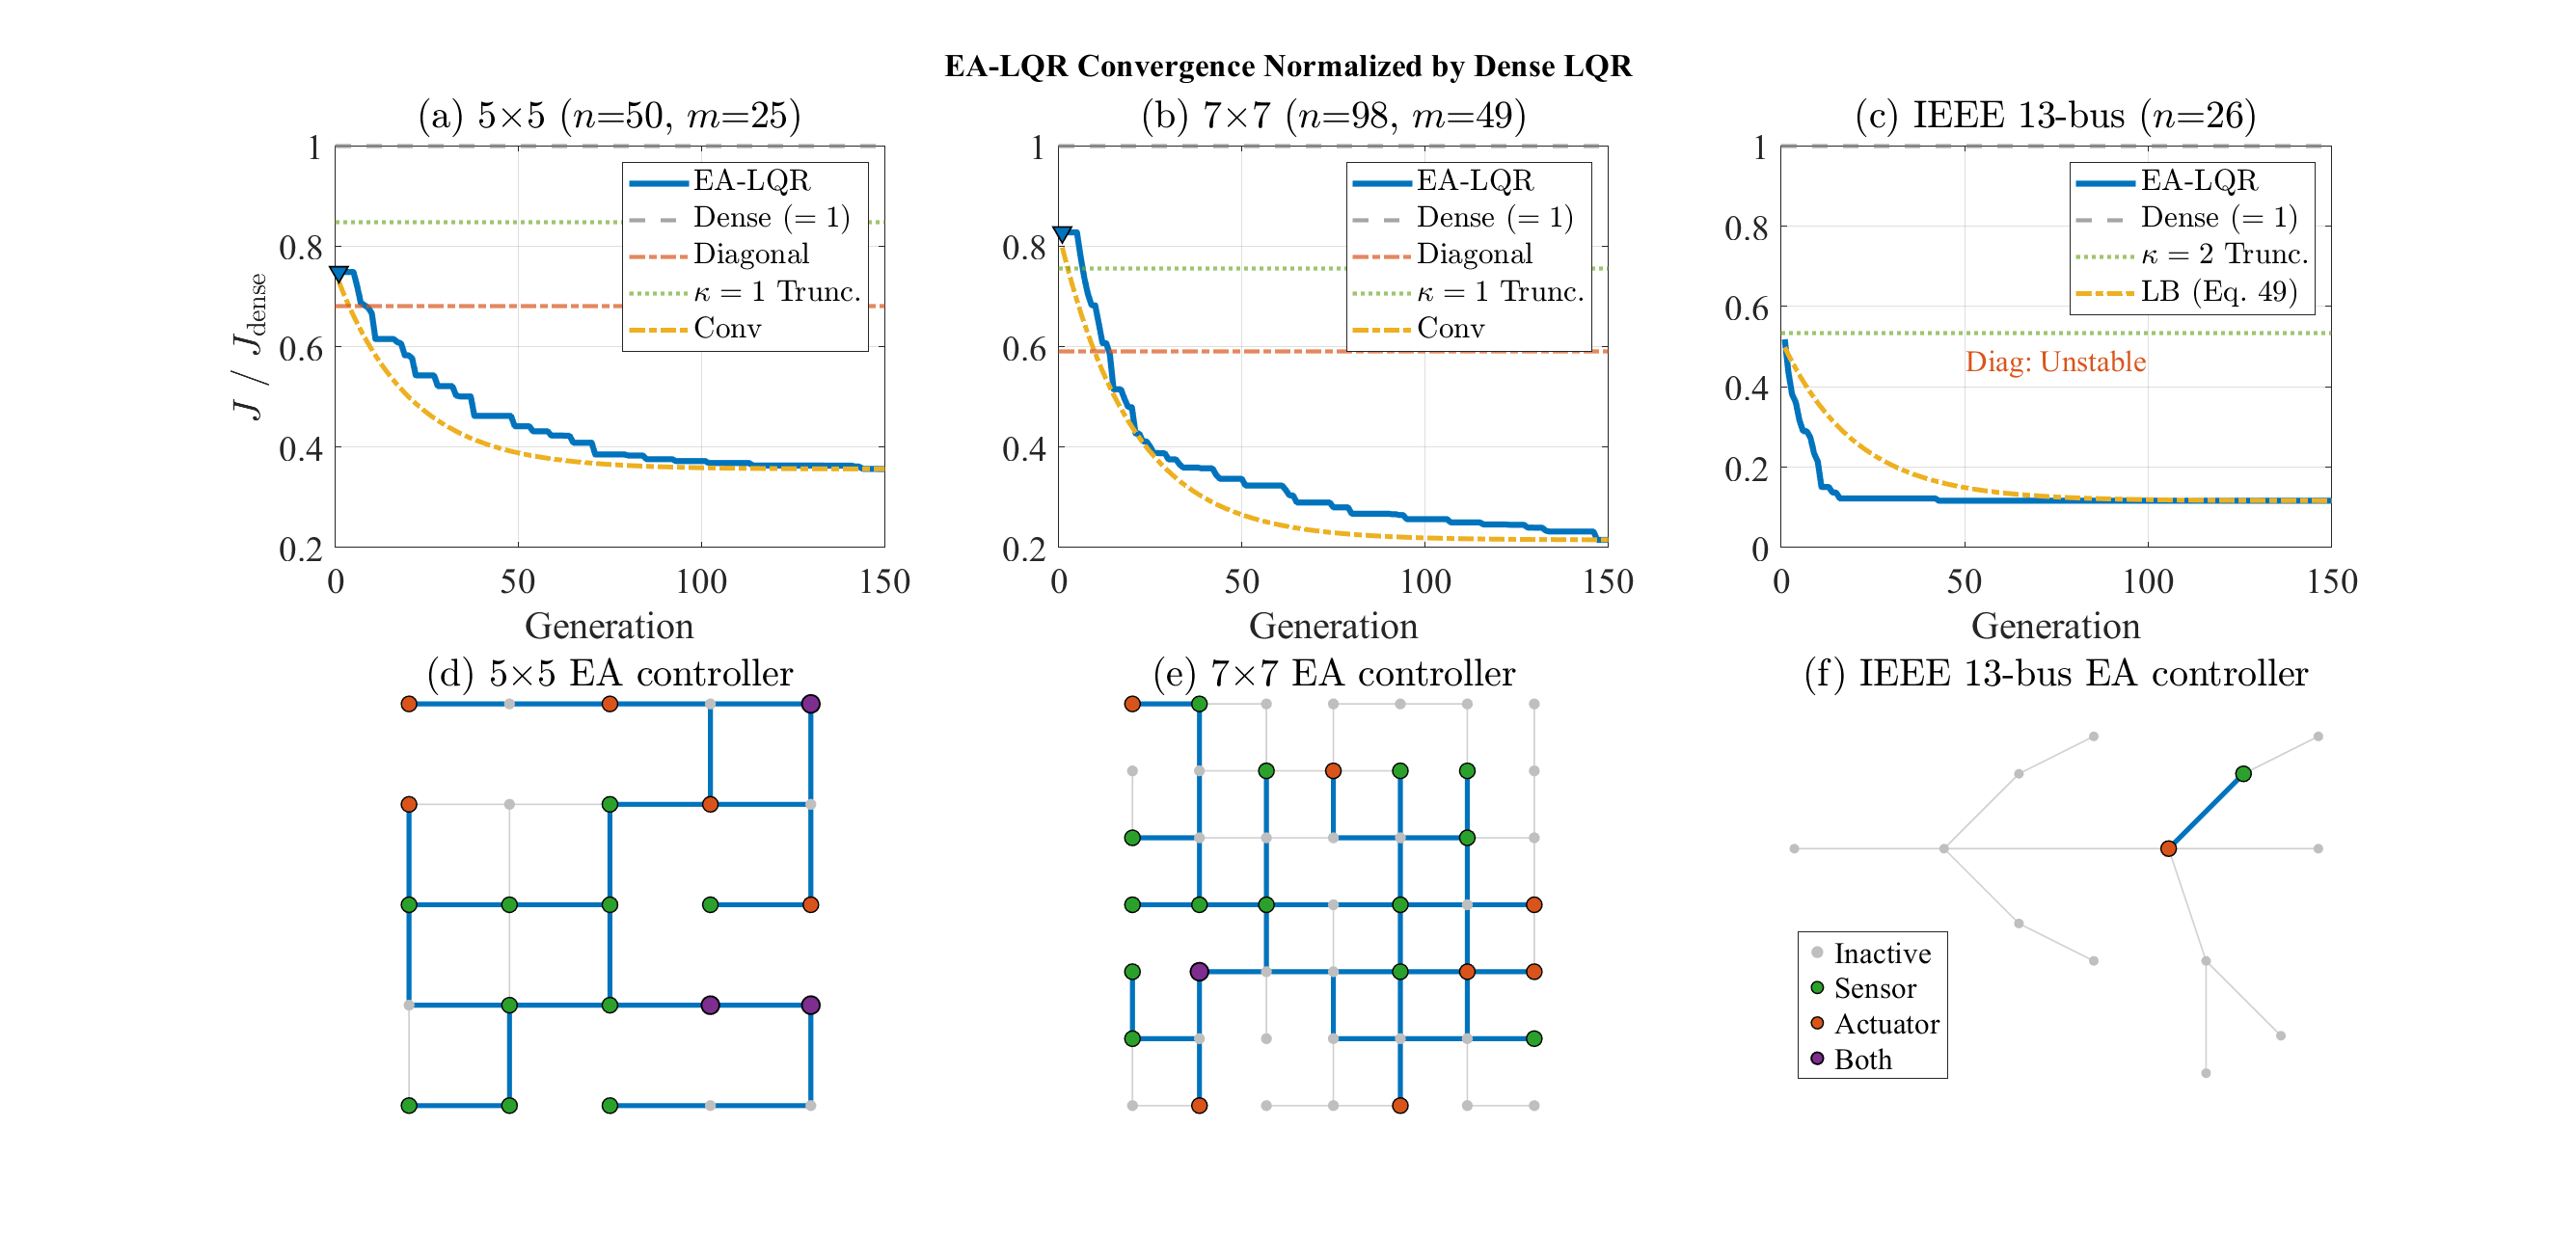
\includegraphics[width=\linewidth]{results/perf_bounds_convergence.png}
    \caption{Normalized EA convergence ($J/J_{\mathrm{d}}$) across grid sizes. Gray dashed: dense LQR ($=1$); orange dash-dotted: diagonal LQR. Triangle: generation at which EA first beats dense LQR. Shaded: $\pm 1\sigma$ over 3 seeds.}
    \label{fig:perf-conv}
  \end{minipage}
  
\end{figure*}

For the stability repair algorithm, a $5{\times}5$ grid system ($N_x = 50$, $N_u = 25$) is generated
with topology seed 10 and connection threshold 0.5, then its spectral
radius is scaled to $\rho(A) = 1.1$.
EA parameters match Table~\ref{tab:sim_params}, with 10 independent
EA seeds $\{1,10,15,20,25,30,35,40,45,50\}$.
$Q = I_{50}$, $R = I_{25}$, $w_c=0.05$, $w_a=0.4$, $w_s=0.2$,
$\alpha=0$. $\bar{\rho} = 0.95$. The result is as follows:
\begin{figure*}[t]
    \centering
    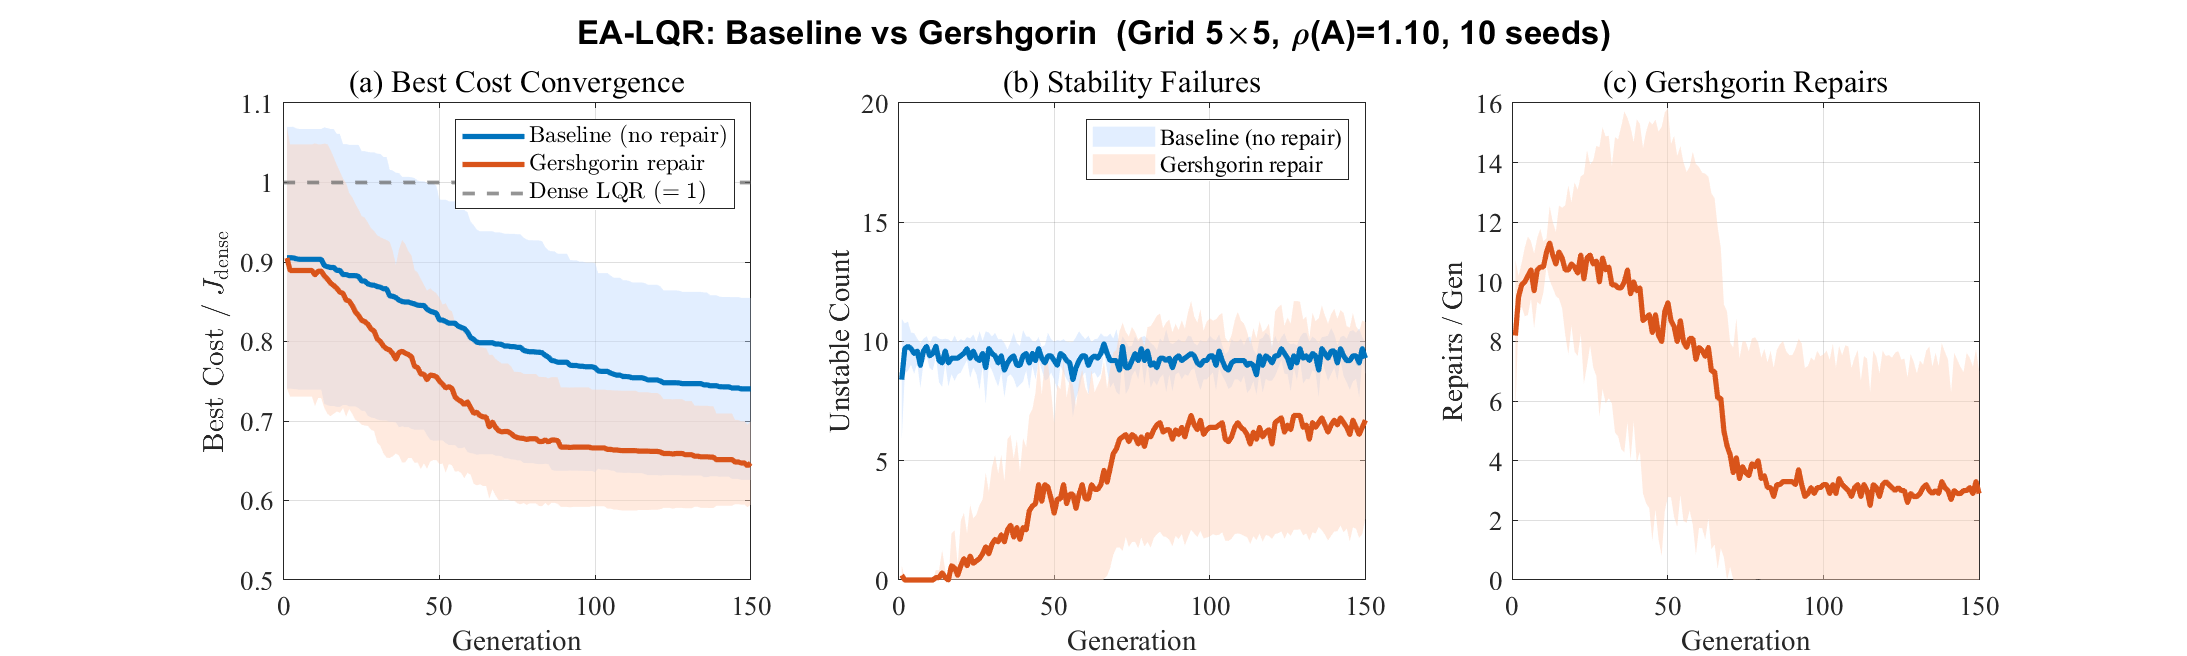
\includegraphics[width=\textwidth]{results/gers_comparison_grid5_unstable_10seeds.png}
    \caption{Average cost, unstable individual controllers and successfully repaired controllers.}
    \label{fig:gers_comparison}
\end{figure*}
Based on the figure \ref{fig:gers_comparison}, EA with Gershgorin repair shows fast initial repair activity that eliminates       
  stability failures by first several generations, after which its effect decays to zero. The convergence rate is almost the same with pure EA, as the repaired $\theta_{rep}$ substituted the unstable ones and  $\theta$ with best fitness are still maintained.
% ------------------------------------------------------------------------

The observations emerge:
\textbf{(i) EA always improves over both baselines.}
Across all grid sizes, EA achieves $J/J_{\mathrm{d}}<1$,
reducing cost by 47--72\% over dense LQR
and 28--52\% over diagonal LQR (Fig.~\ref{fig:perf-conv}).
dense LQR suffers from excessive structural penalties
($J_{\mathrm{struct}} \gg J_{\mathrm{perf}}$),
while diagonal LQR pays a heavy LQR performance penalty
due to the loss of inter-node feedback.
EA balances both components through joint optimization
of the LQR optimization, actuator mask, and sensor mask.

\textbf{(ii) The advantage grows with system dimension.}
As $n$ increases, the d controller's structural cost
scales as $O(mn)$ while diagonal cost stays $O(m)$.
EA exploits the expanding combinatorial space to find
increasingly efficient s topologies,
widening the gap to both baselines.



\bibliography{cit}
\bibliographystyle{IEEEtran}




\end{document}
